\documentclass[a4paper]{article}
\usepackage{geometry}
\usepackage{graphicx}
\usepackage{booktabs}
\usepackage{siunitx}
\usepackage{amsmath}
\usepackage{amssymb}
\usepackage{amsfonts}
\usepackage{enumerate}
\usepackage{multirow}
\usepackage{indentfirst}
\usepackage{rotating}
\usepackage{float}
\usepackage{subfigure}
\usepackage{mathtools}
\usepackage{listings}
\usepackage[cache=false]{minted} 
\usepackage{setspace}
\usepackage[breaklinks,colorlinks,linkcolor=black,citecolor=black,urlcolor=black]{hyperref}
\usepackage{textpos}

\newcommand{\HRule}{\rule{\linewidth}{0.35mm}}

\geometry{top=1in, bottom=1in,left=1.05in, right=1.05in}

\setlength{\parindent}{2em}

\linespread{1.2}

\begin{document}
\setlength{\baselineskip}{18pt}{

\begin{titlepage}

\begin{center}


\includegraphics[height=0.6in]{logo.png}
\HRule \\[0.3cm]
\textsc{\large VE401}\\[0.3cm]
\textsc{\Large Probabilistic Methods in Engineering}\\[0.1cm]

\HRule \\[1.2cm]

\textsc{{\huge Project II}}\\[0.4cm]
\sc{{\large Police Shootings in the United States}}

\vspace{0.3em}
\textit{Analysis of Fatal Police Shooting with Statistic Methods}

\ \\[1.7 cm]

\textbf{\emph{\Large Group 9}}\\[0.3cm]
 %表用三线表!
\begin{figure}[h]
    \hspace{3cm}
    \begin{minipage}{0.4\textwidth}
        \large
        \textbf{\emph{Name:}}\\[0.3cm]
        {Junjie \textsc{Zhang}} \\ 
        {Yimin \textsc{Jiang}} \\
        {Hanyu \textsc{Wang}} \\
        {Yan \textsc{Sun}} \\ 
        {Wenyi \textsc{Cai}} \\ %填上名字
        
    \end{minipage}
    ~
    \begin{minipage}{0.4\textwidth}
        \large
        \textbf{\emph{Student Number:}}\\[0.3cm]
        {517021911128}\\
        {517370910111}\\
        {517370910174}\\
        {517370910147}\\ 
        {516370910139}\\ %填上学号
    \end{minipage}
\end{figure}
\ \\[1.6cm]
\begin{minipage}{0.4\textwidth}

\emph{\textbf{Instructor:}}\\
\Large{Dr. Horst \textsc{Hohberger}}

\end{minipage}\\[1.6cm]
{\large \today}
\end{center}

\end{titlepage}
\newpage

\fontsize{12pt}{\baselineskip}\rm{
\begin{center}
\textbf{{\LARGE Abstract}}
%把你的part做的事情写上
\end{center}
\par{This paper aims to analyze the pattern of \textbf{fatal police shooting} in the US by statistic methods. First, the source of data will be paraphrased and processed; an intuitive graph will be sketched to show the number of fatal police shooting each day between January 1\textsuperscript{st}, 2015 and December 31\textsuperscript{st}, 2018. Next, we apply the knowledge of \textbf{Goodness-of-Fit test} to show that the occurrence of police shootings in the US follows a \textbf{Poisson distribution}. The derivation and numerical values for the \textbf{confidence interval} of the parameter $k$ for the Poisson distribution will also be given in a latter section. Then, we will go deep into the data to see whether the number of police shootings has a dependence on weekdays. Finally, by using \textbf{linear regression}, we will predict the pattern of police shootings in 2019 based on the data between 2015 and 2018, and the actual condition so far turns out to be very close to our prediction.}
\ \\
\ \\
{\small\textbf{Keywords: Fatal Police Shooting, Poisson Distribution, Linear Regression, Confidence Interval, Goodness-of-Fit Test}}

\newpage

\tableofcontents
\newpage

\section{Introduction}
%介绍一下背景,然后引入下
\subsection{Background}
Shooting accident in the US is a frequenter that occupies the headlines of various news medias, and people especially care about whether innocent civilians are shot or killed by a police officer in a specific accident. News medias tend to report those accidents in which many innocent civilians, say, more than 6, are shot or killed by the police, which may lead to the distrust of the public towards the law enforcement capacity of the police. It's true that such unpremeditated injury accidents are misery for every innocent victim, however, for the benefit of the whole society, we may wish to investigate into these striking numbers and find whether there are hard evidences showing that the police are doing a worse job than before.

In this paper, we generally follow the structure of the article \emph{London murders: a predictable pattern?} by David Spiegelhalter and Arthur Barnett [4]. The data from January 1\textsuperscript{st}, 2015 to February 13\textsuperscript{rd}, 2019 for the occurrence of fatal police shootings in the US is obtained from the \emph{Database of Fatal Police Shootings} of the Washington Post [3].

\subsection{Problem Statement}
Though the occurrence of each individual fatal police shooting accident is random, we would expect that the overall pattern may follow a specific distribution. By applying statistics methods, we would be able to illustrate that the occurrence of a large number of victims in a specific police shooting accident is an unusual event but actually not surprising to see during a three-year period. We will also probe into aspects such as how often we would expect days with certain number of fatal police shootings, and the correlation between fatal police shootings and weekdays. The general objective of our analysis is to let the public have a clearer understanding of the pattern of occurrence of fatal police shootings, and avoid unnecessary distrust towards the service ability of the police due to the news report of certain tragedies.

\newpage
\section{Nomenclature} 
% 把一些常用的符号,没有的添加进来,不是常用的就在用前声明就好了
The common variables and concepts that will be used in the paper are listed in Table \ref{NOC} below. Other symbols that are used only once will be described later.
\begin{table}[H]
    \centering
    \begin{tabular}{cl}
         \hline
\textbf{Nomenclature}& \textbf{Full name} \\
\hline\hline
FPS & Fatal Police Shootings\\
d.o.f & Degrees of Freedom\\

$\alpha$ & Level of Significance\\
$k$ & Parameter of Poisson Distribution\\
$X$ & The random variable to be researched. It's Distribution Depends\\
$Y$ & Predictor unless Specified\\
$\chi_{\gamma}^2$ & Random Variable Which Follows Chi-squared Distribution with d.o.f $\gamma$\\
$\chi_{\alpha,\gamma}$ & Value that CDF of Chi-squared Distribution with d.o.f $\gamma$ Achieves 1-$\alpha$\\
\hline
    \end{tabular}
    \centering
    \caption{Nomenclature}
    \label{NOC}
\end{table}

\newpage
\section{Source of Data and ``Fatal Police Shooting"}
\par{In this section, the source of the data will be summarized and the official definition for the terminology used in this paper will be given.}
\subsection{Source of Data}
\par{According to the statement in [1], the database is complied by \emph{Washington Post} and the data comes from news report, publication, social media, and contributes from public by emails.}
\subsection{``Fatal Police Shooting"}
\par{According to the statement in [1], "fatal police shootings" are accidents in which a police officer, in the line of duty, shoots and kills a civilian.}


\newpage
\section{The Pattern of Fatal Police Shootings}
\par{In this section, a similar version of Figure 1 in [4] will be created with the help of \textbf{Mathematica}}.
\par{We processed the data from the database provided in [3] by \textbf{Matlab}. The figure aims to show the number of fatal police shootings each day over this 3-year period, and we just treat February $29^{th}$ as a normal point in x-axis, which can be seen in Figure 1.}
\begin{figure}[h]
    \centering
    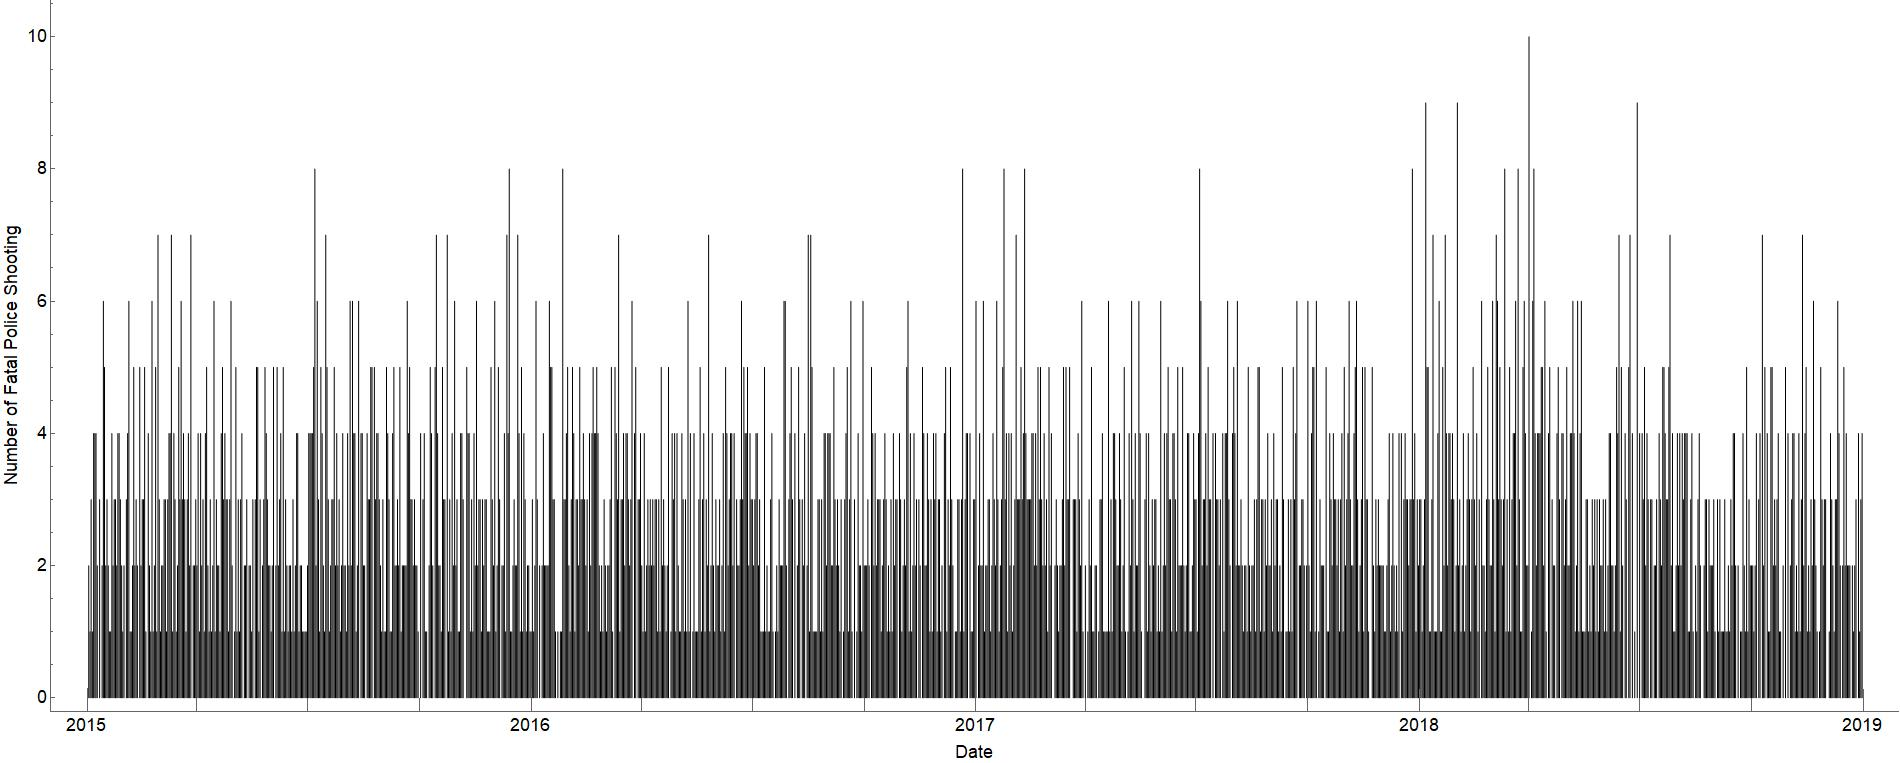
\includegraphics[width = 17cm]{F1.jpg}
    \caption{Number of FPS recorded each day between January $1^{st}$,2015 and December $31^{st}$,2018}
    \label{f1}
\end{figure}

From the figure above, it's hard to tell the overall pattern of the fatal police shootings. However, considering that we are dealing with the whole America population of over 300 million, we would expect that fatal police shootings happen as independent events, and then we can make predictions about the overall pattern based on the data over 3 years in the following sections.

\newpage
\section{Analysis on the Distribution of Daily FPS}% 标题换成内容
In this section, we will discuss whether the number of days with no shooting, one shooting and so on are predictable. We start with the assumption that the fatal police shootings are random events, then the number of shootings happen in three years should follow a Poisson distribution. Therefore, it is constructional to test whether the data follows a Poisson distribution.

First, we abstract the data from 2015 to 2018 and count the number of days with respect to the number of shooting that happen per day. We have the data in Table \ref{ta1}.
\begin{table}[h]
\centering
    \begin{tabular}{c|cccccccccccc}
    \hline
    number of murders & 0 & 1 & 2 & 3 & 4 & 5 & 6 & 7 & 8 & 9 & 10 & $\geq$11\\
    \hline
    \hline
    number of days & 108 & 287 & 324 & 310 & 227 & 116 &53 &21 & 11 & 3 & 1 & 0\\
    \hline
    \end{tabular}
    \caption{The number of days with respect to  shootings that happen per day}
    \label{ta1}
\end{table}

Applying the maximum likelihood estimator, we have the estimator $\hat{k}$ for $k$
\begin{equation}
    \hat{k} = \bar{X} = \sum x\cdot P[X=x] = 2.699
\end{equation}

Since our data covers 1461 days, the expected number of days with certain number of shootings can be calculated as,
\begin{equation}
    E_i = \frac{e^{-k}k^{\lambda_i}}{\lambda_i!}\cdot 1461
\end{equation}
\par{We re-divide the data into different categories to meet the requirements of performing Goodness-of-Fit test and hold data in Table \ref{aaa}. Then we plot the histograms, which is a recreated version of Figure 2 in [4] as shown in Figure 2.}
\begin{table}[h]
\centering
    \begin{tabular}{c|cccccccccc}
    \hline
     & 0 & 1 & 2 & 3 & 4 & 5 & 6 & 7 & 8 & $\geq$9\\
    \hline
    \hline
    $O_i$ & 108 & 287 & 324 & 310 & 227 & 116 &53 &21 & 11 & 4\\
    $E_i$ & 98.3 & 265.3 & 358.0 & 322.1 & 217.3 & 117.3 & 52.8 & 20.3 & 6.9 & 2.8\\
    \hline
    \end{tabular}\\
\caption{The expected value and the observed value of the number of days.}
\label{aaa}
\end{table}
\newpage
\begin{figure}[h]
    \centering
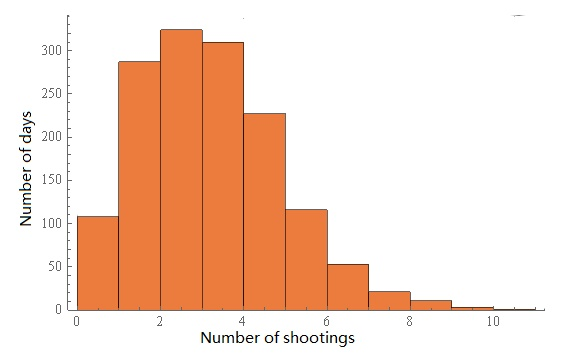
\includegraphics[width = 7.3cm]{figure3-1}
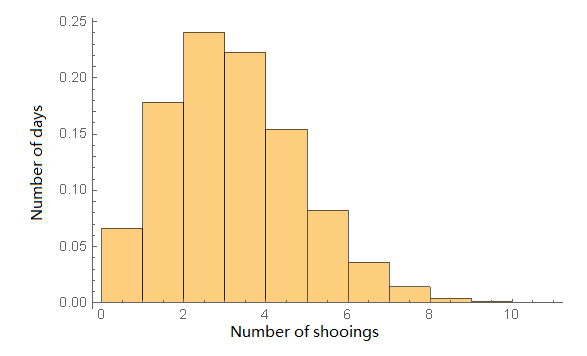
\includegraphics[width = 7.3cm]{figure3-2.png}
     \caption{The observed value(L) and the expected value(R) of the number of days.}
    \label{f1}
\end{figure}

Now, we perform the Goodness-of-Fit test for a discrete distribution. We set up the null hypothesis to be:
    \begin{align*}
    \centering
    H_0: & \textrm{the number of days follows a Poisson distribution with parameter}
    \\& \textrm{$k = 2.699$.}
    \end{align*}

According to the definition, we have the statistic:
\begin{equation}
    \sum_{i=1}^{k} \frac{(O_i-E_i)^2}{E_i}
\end{equation}
, which follows a chi-squared distribution with $k - 1 - m$ degrees of freedom, where $m$ is the number of parameter that we are estimating. Therefore, since we have only one parameter to estimate, which is $k$, and the significance level is set to be $\alpha = 0.05$, we have,
\[X^2 = \sum_{i=1}^{k} \frac{(O_i-E_i)^2}{E_i} \sim \chi_{8}^2\]

Now, we calculate the statistic of our sample
\begin{align*}
    X^2 &= 0.957+1.775+3.229+0.455+0.433\\
    &\ \ +0.014+0.001+0.083+2.436+0.514 \\
           &= 10.136
\end{align*}
\par{And by looking into the table of chi-square distribution, we have the value}
\[\chi_{0.05,8}^2 = 15.507.\]
\par{Since $X^2 = 10.136 < 15.507 = \chi_{0.05,8}^2$, we fail to reject $H_0$ at $5\%$ level of significance. Therefore, we have no evidence that the number of days with various fatal police shootings does not follow a Poisson distribution with parameter $k = 2.699$.}

\newpage
\section{Test for Weekday Dependency}% 标题换成内容
In this section, we mainly discuss whether the number of shootings depends on weekdays. Based on the data, we have the number of shootings with respect to the weekday as shown in Table 4. We plot the histogram below to show the distribution intuitively.

\begin{table}[h]
\centering
    \begin{tabular}{cccccccc}
         \hline
         Mon & Tue & Wed & Thu & Fri & Sat & Sun \\
         \hline
         \hline
         538 & 600 & 633 & 590 & 584 & 533 & 576\\
         \hline
    \end{tabular}\\
    \caption{The number of shootings with respect to weekdays.}
\end{table}

\begin{figure}[h]
    \centering
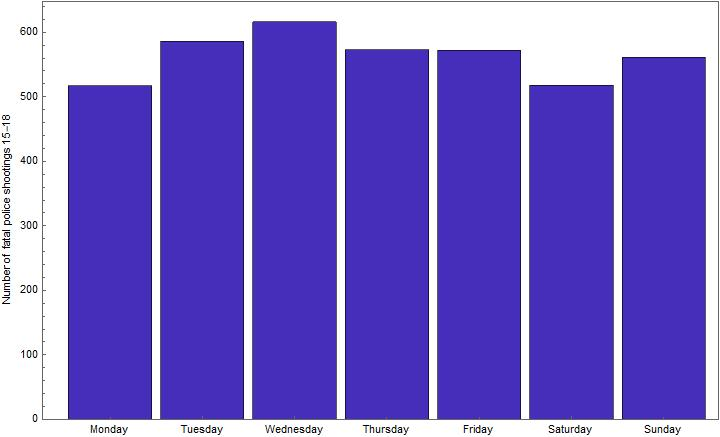
\includegraphics[width = 10cm]{1}
     \caption{The expected value and the observed value of the number of days.}
    \label{f1}
\end{figure}
We are going to test whether those seven numbers indicate a uniform distribution of fatal police shootings. Assuming a uniform distribution (the difference of the number of different weekdays is negligible since three year is quite a long period), that is:
\begin{equation}
    \textrm{P[Mon] = P[Tue] = P[Wed] = P[Thu] = P[Fri] = P[Sat] = P[Sun] = }\frac{1}{7}
\end{equation} 
\par{Now, since the total number of days is 1461, we can easily calculate the expected value according to the uniform distribution. Table 5 combines the observed value and the expected value for each weekday.}

\begin{table}[h]
\centering
    \begin{tabular}{c|cccccccc}
         \hline
         & Mon & Tue & Wed & Thu & Fri & Sat & Sun \\
         \hline
         \hline
         $O_i$ & 538 & 600 & 633 & 590 & 584 & 533  & 576\\
         $E_i$  & 579.1 & 579.1 & 579.1 & 579.1 & 579.1 & 579.1 & 579.1\\
         \hline
    \end{tabular}\\
    \caption{The observed and expected values of the weekday dependency.}
\end{table}
Similarly, we perform the Goodness-of-Fit test for a discrete distribution. We set up the null hypothesis to be:
   \begin{align*}
    \centering
    H_0: & \textrm{The number of fatal police shootings are uniformly distributed}
    \\& \textrm{on each weekday.}
    \end{align*}
\par{According to the definition, we test the statistic}
\[\sum_{i=1}^{k}\frac{(O_i-E_i)^2}{E_i}\]
, which follows a chi-square distribution with $k-1-m$ degrees of freedom. In this question we have no parameter to estimate, therefore $m = 0$, thus the degrees of freedom is $k-1=6$. The significance level is set to be $\alpha = 0.05$, so we have
\begin{equation}
    X^2 = \sum_{i=1}^{k}\frac{(O_i-E_i)^2}{E_i}\sim \chi_{6}^2
\end{equation}
\par{To conduct this test, we first calculate the statistic of our sample}
\begin{align*}
    X^2 &= 0.016 + 2.917 + 0.754 + 5.017 + 0.205 + 0.041 + 3.670\\
           &= 12.62.
\end{align*}
\par{By looking into the table of chi-square distribution we have the value}
\[\chi_{0.05,6}^2 = 12.592\]

Since $X^2 = 12.62>12.592 = \chi_{0.05,6}^2$, we decide to reject the hypothesis at the significance level of $5\%$. Therefore, though intuitively we believe that the number of fatal police shootings should be irrelevant with weekdays, we have no evidence to say that the number of police shootings are uniformly distributed with respect to weekdays.

\newpage
\section{Confidence Interval of $k$}% 标题换成内容
\par{In this section, we'll derive the confidence interval of parameter $k$ based on data from year 2015 to 2018. Then we'll calculate confidence intervals for given $\alpha$ and comment on them.}
\subsection{Formula for Confidence Interval}
\par{We have the random variable X which follows a Poisson distribution with expectation $\textrm{E[X]}=k$ and variance $\textrm{Var X}=k$. In our case, since we have a very large sample size, by the central limit theorem, we can assume that $\hat{k}$ is approximately normally distributed with mean $k$ and variance $k/n$. Hence, the statistic}
\begin{equation*}
    \frac{\hat{k}-k}{\sqrt{k/n}}
\end{equation*}
is approximately standard-normally distributed.
\par{With this condition, a 100(1-$\alpha$)\% confidence interval for $k$ is given by}
\begin{equation*}
\^{k}\pm z_{\alpha/2}\sqrt{k/n}
\end{equation*}
\par{Here, the problem occurs that the confidence interval depends on the unknown parameter $k$, which we are trying to estimate. For this specific case, since our sample is really large, we may presume that the difference between $k$ and $\hat{k}$ is negligible. Therefore, we can just substitute $k$ by $\^{k}$ for approximation. And after we get the confidence interval of $k$, we will plug it in back to see whether this approximation can work.}
\begin{equation}
\^{k}\pm z_{\alpha/2}\sqrt{\^{k}/n}
\end{equation}
\par{Considering the estimator $\^{k}$ :}
\begin{equation*}
    \^{k} = \bar{X} = \bar{x}_{2015-2018} =  2.69884
\end{equation*}
\par{Considering the leap year, the size of our sample is}
\begin{equation*}
    n = 365 \times 4 + 1 =  1461
\end{equation*}
\par{Now, we plug in the data and the result is given by}
\begin{equation}
    k=2.69884\pm z_{\alpha/2}\cdot \sqrt{2.6988/1461}=2.69884\pm 0.04298\cdot z_{\alpha/2}
\end{equation}
\subsection{Values of Confidence Interval for Given $\alpha$}
\par{We plug in some common $\alpha$ to see the confidence interval with different levels of significance. These confidence intervals of k with certain $\alpha$ are shown in Table \ref{cfi}}.
\begin{table}[h]
\centering
    \begin{tabular}{c|c}
         \hline
$\alpha$& 100(1-$\alpha$)\% confidence intervals of $k$\\
\hline
\hline
        0.001&[2.55741, 2.84027]\\
          0.01&[2.58813, 2.80955]\\

         0.02&[2.59885, 2.79883]\\

         0.05&[2.61460, 2.78308]\\
 
         0.1&[2.62814, 2.76954]\\
         \hline
    \end{tabular}
\caption{100(1-$\alpha$)\% confidence interval of $k$.}
\label{cfi}
\end{table}
\par{To verify the performance of our model, we notice that the confidence intervals are relatively narrow and the difference between $\^{k}$ and $k$ can really be neglected for common cases. Even for the 99.9\% confidence interval, we can see that the maximum difference between $\^{k}$ and $k$ is 0.28286, which is considerable small. Hence, we consider our model works well for these data.}
\newpage

\section{Analysis on the Distribution of Fatal Police Shooting in 2019}% 标题换成内容
\par{In this section, we'll test whether number of fatal police shootings in 2019 follows a Poisson distribution.}
\par{Based on the database in [3], we get data of 2019 from Jan.$1^{st}$ to Feb.$13^{rd}$, which is 44 days in total. In other words, we only have sample with size $n = 44$.}
\par{Based on these data, the estimator for parameter $k$ is:}
\begin{equation}
    \^{k} = \Bar{X} = \bar{x}_{2019} = 2.477
\end{equation}
\par{Then, to test whether the data follows a Poisson distribution, we set the null hypothesis as :}
    \begin{align*}
    H_0: & \textrm{ the number of FPS during the period from Jan. $1^{st}$ to Feb. $13^{rd}$ in 2019}
    \\& \textrm{ follows a Poisson distribution with parameter k = 2.477.}
    \end{align*}
    \par{Since the size of sample $n$ is 44,  the expected values for daily fatal police shootings are calculated by}
    \begin{equation}
    E_i = \frac{e^{-k}k^{\lambda_i}}{\lambda_i!}\cdot 44
\end{equation}
and shown in Table \ref{ff}.
\par{Then, divide the data in to proper categories to meet the criteria of Good-of-Fitness Test, which is shown in Table \ref{ff}.}
\begin{table}[h]
    \centering
    \begin{tabular}{l|ccccc}
    \hline
                 & 0            & 1            & 2             & 3            & \geq4           \\ \hline\hline
$E_i$           &3.696	&9.154	&11.338	&9.361	&     10.451         \\ 
$O_i$           & 3            & 14           & 8             & 7            & 12             \\ \hline
\end{tabular}
\caption{Expected and observed number of days for certain number of FPS from $Jan.1^{st}$ to $Feb.13^{rd}$ in 2019.}
\label{ff}
\end{table}

\par{For $N=5$ categories, the static}
\begin{equation}
    X^2= \sum_{i=1}^{5} \frac{(O_i-E_i)^2}{E_i} = 4.504
\end{equation}
follows a chi-squared distribution with $N-1-m=5-1-1=3$ degrees of freedom. We set the significance level to be $\alpha=0.05$.
Then, since $\chi^2_{0.05,3} = 7.815>X^2$, we fail to reject $H_0$ at significant level 0.05.
\par{In conclusion, we have no evidence that the number of fatal police shooting during the period from Jan.$1^{st}$ to Feb.$13^{rd}$ in 2019 does not follow a Poisson distribution with parameter $k = 2.477$. Thus, we believe it follows the Poisson distribution.}
\begin{equation*}
    \
\end{equation*}

\newpage
\section{Prediction of Fatal Police Shootings in 2019}% 标题换成内容
\par{In this section, we will derive Nelson’s formula. Then, the formula is used to obtain 95$\%$ prediction intervals for the number of mass shootings in 2019 based on the data from 2015 to 2018. Finally, the data is plotted along with their prediction intervals.}
\subsection{Deriving Nelson's formula}
\par{First, let $X$ denote the total counts in a sample of size $n$ from a Poisson distribution with mean $\lambda$. Let $Y$ denote the future total counts that can be observed in a sample of size m from the same Poisson distribution. Let $\hat{\lambda}$=$X/n$, we have $\textrm{E}[\hat{\lambda}]=\lambda$, which is an unbiased estimator of $\lambda$. The variance of the estimator is calculated as:}
\begin{equation}
    \textrm{Var }\hat{\lambda}=\frac{1}{n^2}\textrm{Var }X=\frac{\lambda}{n}
\end{equation}
\par{Known that $\textrm{E}[Y]=m\lambda$ and $\textrm{Var }Y=m\lambda$, the expected value of $m\hat{\lambda} -Y$ is given by}
\begin{equation}
    \textrm{E}[m\hat{\lambda}-Y]=\textrm{E}[m\hat{\lambda}]-\textrm{E}[Y]=m\lambda-m\lambda=0
\end{equation}
\par{And the variance of $m\hat{\lambda} -Y$ is given by}
\begin{equation}
    \textrm{Var }(m\hat{\lambda}-Y)=\textrm{Var }m\hat{\lambda}+\textrm{Var }Y=m^2\frac{\lambda}{n}+m\lambda=m^2\lambda(\frac{1}{m}+\frac{1}{n})
\end{equation}
\par{When n is large, the variance can be approximated by substituting $\lambda$ by $\hat{\lambda}$ This will only lead to a very small error when the sample size n is really large.}
\par{According to the central limit theorem, we have that $m\hat{\lambda}-Y$ is approximately normally distributed if the sample size is large. Based on this assumption, we have (m$\hat{\lambda}-Y$)/$\sqrt{\textrm{Var }(m\hat{\lambda}-Y)}$ is a standard normal distribution. Then the prediction interval is given by}
\begin{equation}
[\lceil L \rceil,\lfloor U \rfloor]       with [L,U]=\hat{Y}\pm z_{\alpha/2}\sqrt{m\hat{Y}(\frac{1}{m}+\frac{1}{n})}
\end{equation}
\par{where $\hat{Y}=m X/n$, for $X=1,2,...$, and is 0.5m/n when $X=0$. Above all, we have shown the nelson prediction interval.}%discuss 0.5m/n if time is available. Not important for our cases.
\subsection{Predict the pattern of fatal police shootings in 2019}
\par{Then, with our derived formula, we can now predict the pattern of fatal police shootings in 2019. Since our sample size is large, Nelson's formula is valid. Let $k$ denote the mean of the Poisson distribution of fatal police shootings. Let $X$ be the total counts of fatal police shootings in a sample of size $n$ from 2015-2018. Let $Y$ be the total counts of fatal police shootings in a sample of size $m$ in 2019.  Based on the data, we plug in $\hat{k}$=2.69884, n=1461, m=365, and $\hat{Y}=m\hat{k}=985.0766$ to the formula to get the prediction interval of Y with 95$\%$ confidence interval as: }
\begin{equation}
\begin{split}
[L,U]&=\hat{Y}\pm z_{\alpha/2}\sqrt{m\hat{Y}(\frac{1}{m}+\frac{1}{n})}\\
     &=985.0766\pm1.96\times \sqrt{365\times 985.0766(\frac{1}{365}+\frac{1}{1461})}\\
     &=985.0766\pm68.77\\
\end{split}
\end{equation}
    
\par{Hence, the prediction interval for the total shooting in 2019 is approximately \\ Y=[$\lceil L \rceil,\lfloor U \rfloor$]=[917,1053]. With the help of \textbf{Mathematica}, the graph is plotted. In Figure 4, the plot of the prediction interval is shown. In Figure 5, the plot of the prediction interval in the first 44 days along with the existing data is shown.}
\begin{figure}[H]
    \centering
    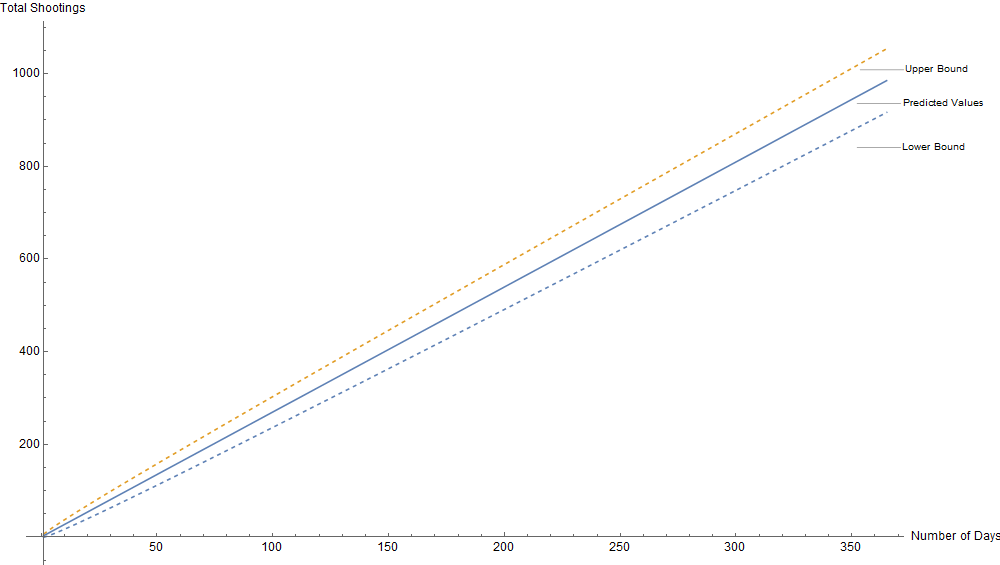
\includegraphics[width = 15cm]{figure7-1}
    \caption{The prediction interval of the number of mass shootings in 2019.}
    \label{f1}
\end{figure}
\begin{figure}[H]
    \centering
    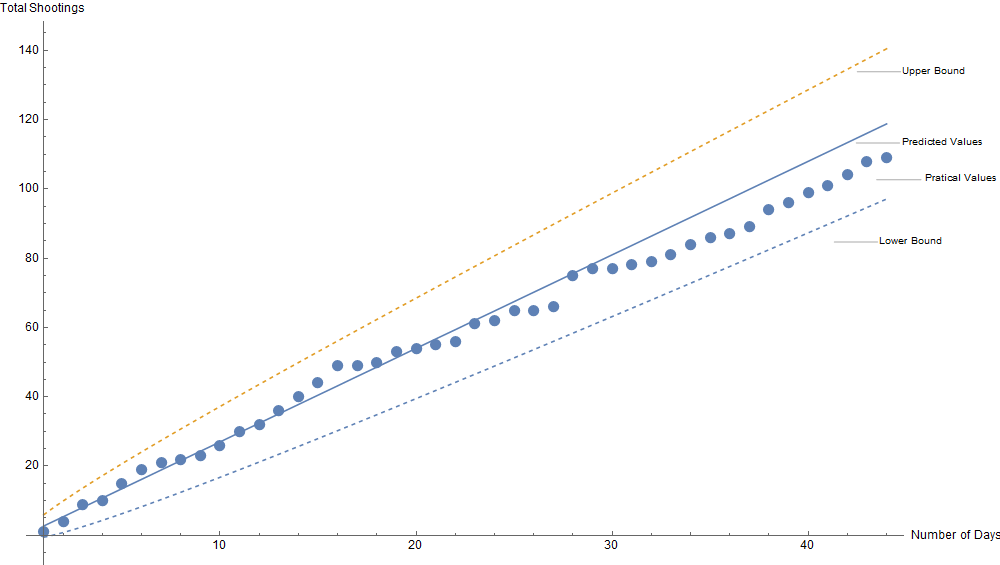
\includegraphics[width = 15cm]{figure7-2}
    \caption{The prediction interval in the first 44 days along with the existing data.}
    \label{f1}
\end{figure}

\newpage

\section{Conclusion}
%把你的part做的事情写上
\par{In this paper, fatal police shootings in the US are discussed by statistic methods. After exploring the pattern of fatal police shootings between January  1\textsuperscript{st}, 2015 and December 31\textsuperscript{st}, 2018, we estimate that the fatal police shooting accidents follow a Poisson distribution with parameter $k = 2.70$. Then, we test the dependency of the number of police shootings on the weekday, and find that police shootings seem more likely to happen on Wednesday, while less likely to happen on Saturday. Next, we derive the formula for a $(1-\alpha)100\%$ confidence interval for the parameter $k$, which is $\hat{k} \pm z_{\alpha/2}\sqrt{k/n}$. Finally, based on the data from 2015 to 2018, we predict the pattern of fatal police shootings in 2019 by using Nelson's formula, and the existing data for the first 44 days of 2019 falls into the confidence interval of our prediction, which verifies the validity of our prediction. To sum up, there's no hard evidence showing that the police are doing a worse job than before, so there's actually no need to feel panic for the shocking numbers of fatal police shootings reported by news medias.
}

\newpage
\section{Appendix}
\subsection{Data Pre-processing}
\begin{minted}[mathescape,
               linenos,
               numbersep=5pt,
               gobble=2,
               frame=lines,
               framesep=2mm]{matlab}
    load('rawData');
    
    Date = num2str(rawData);
    data = [];
    Y = zeros(size(Date,1),1);
    M = zeros(size(Date,1),1);
    D = zeros(size(Date,1),1);
    
    for ii = 1:size(Date,1)
        Y(ii) = str2num(Date(ii,[1:4]));
        M(ii) = str2num(Date(ii,[5:6]));
        D(ii) = str2num(Date(ii,[7:8]));
    end
    DateP = datenum([Y,M,D]);
    date = datenum([2015 1 1]);
    
    iter = 1;
    num = 0;
    for ii = 1:size(rawData,1)
        if DateP(ii) == date
            num = num+1;
        elseif DateP(ii) == date + 1
            date = DateP(ii,1);
            data = [data;num];
            num = 1;
            iter = iter + 1;
        else
            data = [data;num];
            num = 1;
            for jj = 1:DateP(ii)-date-1
                data = [data;0];
                iter = iter + 1;
            end
            date = DateP(ii,1);
        end
    end
    
    st = datenum([2015 1 1]);
    ed = datenum([2018 12 31]);
    data2 = data([1:ed-st+1]);
    year1 = data([1:datenum([2015 12 31])-datenum([2015 1 1])+1]);
    year2 = data([datenum([2015 12 31])-datenum([2015 1 1])...
    +2:datenum([2016 12 31])-datenum([2015 1 1])+1]);
    year3 = data([datenum([2016 12 31])-datenum([2015 1 1])+...
    2:datenum([2017 12 31])-datenum([2015 1 1])+1]);
    year4 = data([datenum([2017 12 31])-datenum([2015 1 1])+...
    2:datenum([2018 12 31])-datenum([2015 1 1])+1]);
    year5 = data([datenum([2018 12 31])-datenum([2015 1 1])+2:end]);
    csvwrite('year1.csv',year1);
    csvwrite('year2.csv',year2);
    csvwrite('year3.csv',year3);
    csvwrite('year4.csv',year4);
    csvwrite('year5.csv',year5);
    
    Wkd = weekday(DateP);
    csvwrite('Wkd.csv',Wkd);

\end{minted}
\subsection{Recreate Figure 1 in [4]}
\begin{minted}[mathescape,
               gobble=0,
               frame=lines,
               framesep=2mm]{mathematica}
 
    data := Import["dataProcessed.csv", "List"]
    DateListPlot[data, {2015, 1, 1}, PlotStyle -> Black, Filling -> Axis, 
     FillingStyle -> Black, Joined -> False, PlotMarkers -> "", 
     FrameLabel -> {"Date", "Number of Fatal Police Shooting"}, 
     AspectRatio -> 1/2.6, ImageSize -> 1900, 
     Frame -> {{True, False}, {True, False}}]
    \end{minted}
    \subsection{Create Figure 3}
\begin{minted}[mathescape,
               gobble=0,
               frame=lines,
               framesep=2mm]{mathematica}
 BarChart[Apply[Labeled, Reverse[td, 2], {1}], 
 ChartStyle -> {ColorData["Rainbow"][0.1]},  
 FrameTicks -> {{Automatic, None}, {Automatic, None}}, 
 FrameLabel -> {None, "Number of fatal police shootings 15-18"},
 -> {10, GrayLevel[0]}]

\end{minted}
  \subsection{Create Figure 4,5}
  \begin{minted}[mathescape,
               gobble=0,
               frame=lines,
               framesep=2mm]{mathematica}
p1 = Plot[{m*2.69884 - 1.96*(Sqrt[m^2*2.69884*(1/m + 1/1461)]), 
    m*2.69884 + 1.96*(Sqrt[m^2*2.69884*(1/m + 1/1461)])}, {m, 1, 365},
    PlotStyle -> Dashed, PlotLabels -> {"Lower Bound", "Upper Bound"}];
p2 = Plot[{2.69884*m}, {m, 1, 365}, 
   PlotLabels -> {"Predicted Values"}];
Show[p1, p2, AxesLabel -> {"Number of Days", "Total Shootings"}, 
 ImageSize -> 1000, LabelStyle -> {12, GrayLevel[0]}]


p1 = Plot[{m*2.69884 - 1.96*(Sqrt[m^2*2.69884*(1/m + 1/1461)]), 
    m*2.69884 + 1.96*(Sqrt[m^2*2.69884*(1/m + 1/1461)])}, {m, 1, 44}, 
   PlotStyle -> Dashed, PlotLabels -> {"Lower Bound", "Upper Bound"}];
p2 = Plot[{2.69884*m}, {m, 1, 44}, PlotLabels -> {"Predicted Values"}];
p3 = ListPlot[{1, 4, 9, 10, 15, 19, 21, 22, 23, 26, 30, 32, 36, 40, 
   44, 49, 49, 50, 53, 54, 55, 56, 61, 62, 65, 65, 66, 75, 77, 77, 78,
    79, 81, 84, 86, 87, 89, 94, 96, 99, 101, 104, 108, 109}, 
  PlotLabels -> {"Pratical Values"}]
Show[p1, p2, p3, AxesLabel -> {"Number of Days", "Total Shootings"}, 
 ImageSize -> 1000, LabelStyle -> {12, GrayLevel[0]}]
\end{minted}
\newpage
\section{Reference}
\begin{thebibliography}{9}
\bibitem{kj}
K.Krishnamoorthy and J.Peng. Improved closed-form prediction intervals for binomial and Poisson distributions. \emph{Journal of Statistical Planning and Inference}, 141(5):1709-1718, 2011. http://www.sciencedirect.com/science/article/pii/S0378375810005215.

\bibitem{vh}
V. Patil and H. Kulkarni. Comparison of confidence intervals for the Poisson mean: some new aspects. \emph{REVSTAT-Statistical Journal},  10(2):211-227, 2012.

\bibitem{washinton post}
The Washington Post. Fatal force. https://www.washingtonpost.com/graphics/national/police-shootings-2016/. Web. Accessed April 10th, 2019.

\bibitem{da}
D. Spiegelhalter and A. Barnett. London murders: a predictable pattern? \emph{Significance}, 6(1):5-8, 2009. http://onlinelibrary.wiley.com/doi/10.1111/j.1740-9713.2009.00334.x/abstract.

\bibitem{horst}
Horst Hohberger, \emph{VE401,Probabilistic Methods in Eng. Slides}, University OF Michigan - Shanghai Jiao Tong University Joint Institute, Shanghai, China
\end{thebibliography}
}}
\end{document}